\documentclass[../../main/main.tex]{subfiles}
\usepackage{geometry}

\begin{document}
\section{Parameter and Payoff Analysis}

Having established the Nash equilibrium (Section 4), analyzed the game value (Section \ref{sec:game_value}), and proved convergence to FBCP and NLCP (Section \ref{sec:strategic_comparison}), we now explore in greater detail how the parameters $L$ and $U$ affect player strategies and payoffs. This section summarizes key insights and presents visualizations that illuminate the strategic dynamics of LCP. Complete technical proofs are provided in Appendices \ref{sec:parameter_analysis} and \ref{sec:payoff_analysis}.

\subsection{Visualizing Payoffs in Equilibrium}

In Nash equilibrium, each hand combination $(x, y)$ uniquely determines the bettor's payoff. Figure \ref{fig:payoffs} shows how these payoffs vary across the unit square for different values of $L$ and $U$, from strict limits (Fixed-Bet, $L=U=1$) to lenient limits (No-Limit, $U \to \infty$).

\clearpage
\newgeometry{top=0in,left=0.5in,right=0.5in,bottom=0.5in}
\begin{figure}[p]
    \begin{adjustwidth}{-1.25in}{-1.25in}
        \centering
        \begin{minipage}{0.4\textwidth}
            \centering
            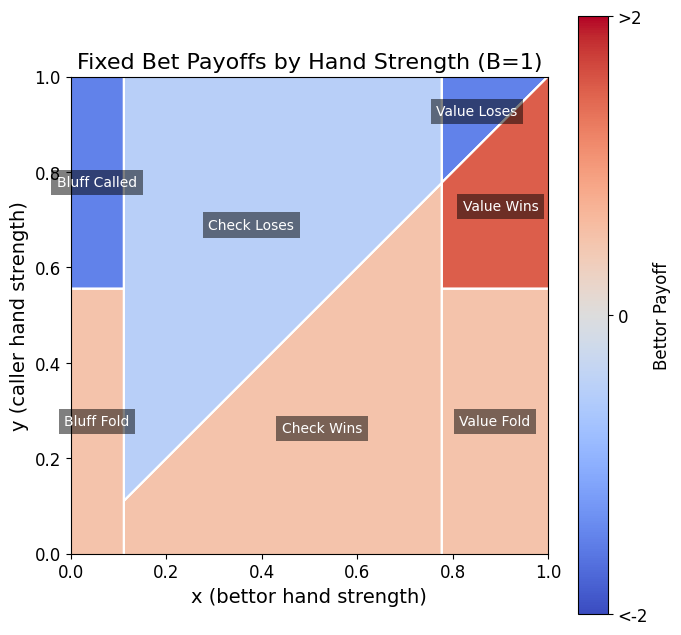
\includegraphics[width=\textwidth]{../payoff_analysis/images/payoffs_1_1.png}
        \end{minipage}
        \hspace{0.05\textwidth}
        \begin{minipage}{0.4\textwidth}
            \centering
            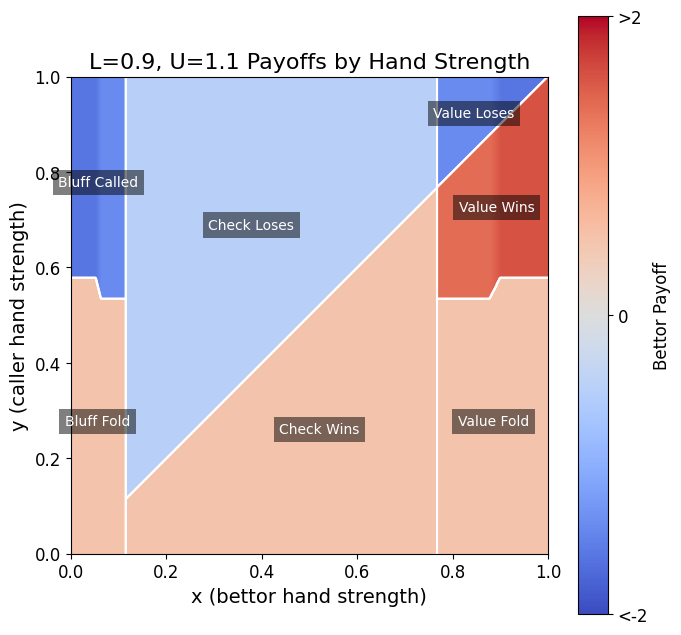
\includegraphics[width=\textwidth]{../payoff_analysis/images/payoffs_0.9_1.1.png}
        \end{minipage}
        \vspace{0.4cm}\\
        \begin{minipage}{0.4\textwidth}
            \centering
            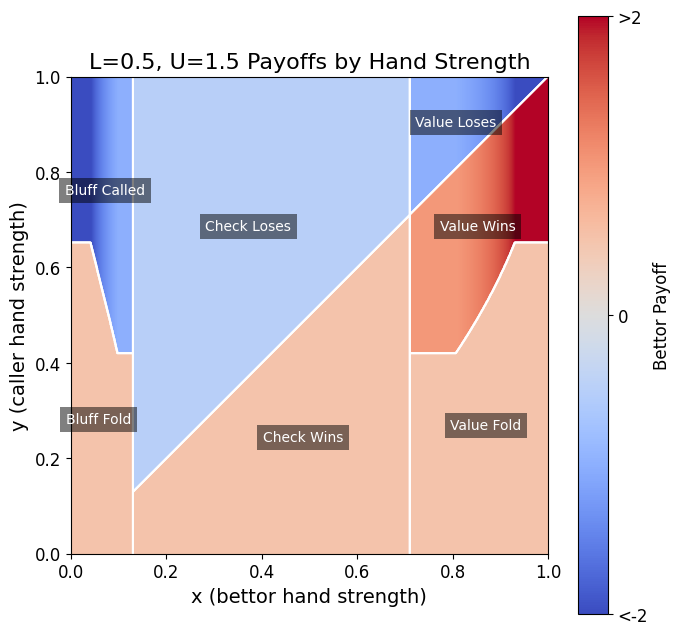
\includegraphics[width=\textwidth]{../payoff_analysis/images/payoffs_0.5_1.5.png}
        \end{minipage}
        \hspace{0.05\textwidth}
        \begin{minipage}{0.4\textwidth}
            \centering
            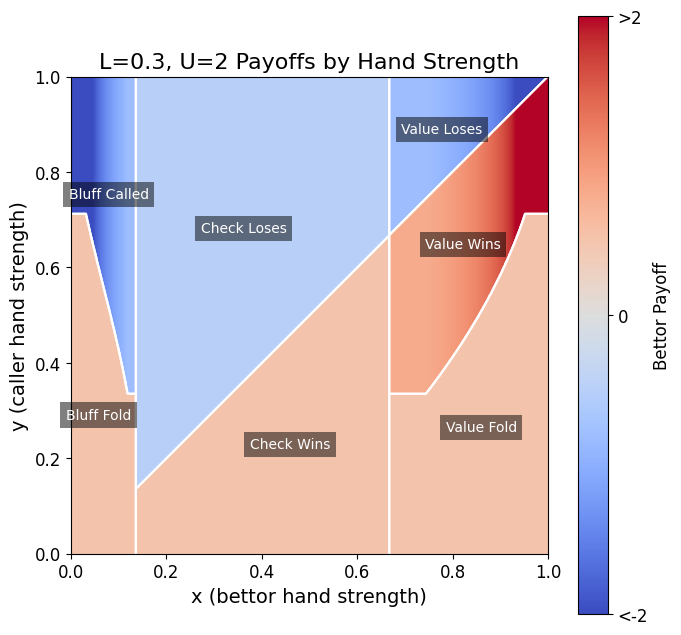
\includegraphics[width=\textwidth]{../payoff_analysis/images/payoffs_0.3_2.png}
        \end{minipage}
        \vspace{0.4cm}\\
        \begin{minipage}{0.4\textwidth}
            \centering
            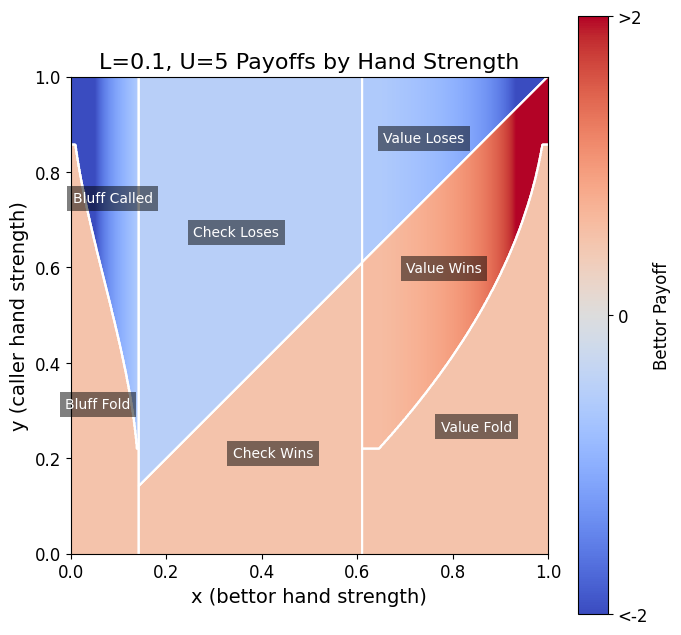
\includegraphics[width=\textwidth]{../payoff_analysis/images/payoffs_0.1_5.png}
        \end{minipage}
        \hspace{0.05\textwidth}
        \begin{minipage}{0.4\textwidth}
            \centering
            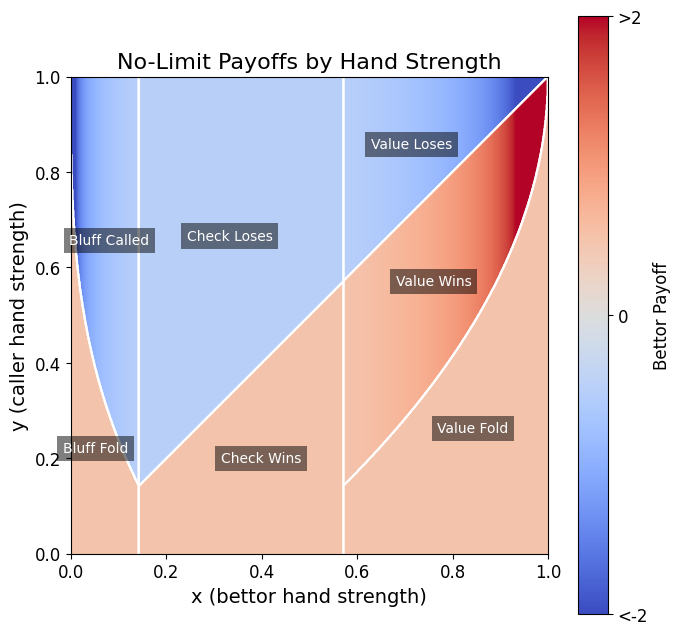
\includegraphics[width=\textwidth]{../payoff_analysis/images/payoffs_0_inf.png}
        \end{minipage}
    \end{adjustwidth}
    \caption{Bettor payoffs in Nash equilibrium as a function of hand strengths $x, y$ for fixed bet size $B=1$ (top left), and No-Limit Continuous Poker (bottom right). Intermediate plots show the payoffs for different values of $L$ and $U$ ranging from strict (fixed bet size $B=1$) to lenient (No limits). Regions are labeled according to the outcome of the game in Nash equilibrium.}
    \label{fig:payoffs}
\end{figure}

\restoregeometry

The visualization reveals that the biggest wins and losses occur when both hands are strong (top right), consistent with real poker intuition. Large payoffs also occur when a very weak bettor bluffs big and gets called by a strong caller (top left). As limits become more lenient, these extreme outcomes become more pronounced but also less likely, since making and calling maximum bets become riskier for both players.

\subsection{Expected Value by Hand Strength}

Beyond specific hand matchups, we can analyze the expected value $EV(x)$ of a bettor hand $x$ averaged over all possible caller hands. This function characterizes how profitable each hand is in equilibrium.

\begin{figure}[h!]
    \centering
    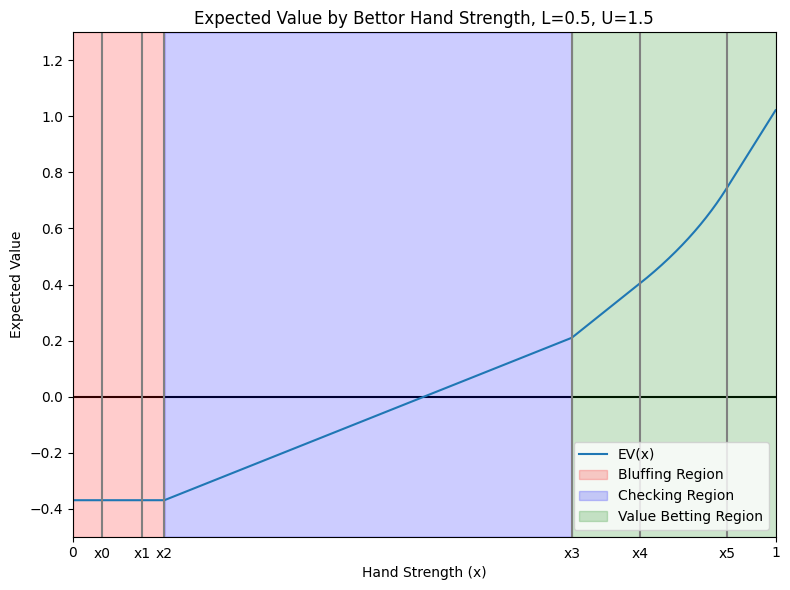
\includegraphics[width=\textwidth]{../payoff_analysis/images/ExpectedPayoffs.png}
    \caption{Expected value of bettor hand strength $x$ in the unique admissible Nash equilibrium for various parameter settings. The bettor's expected value is increasing in $x$ (stronger hands are more profitable), with discontinuities at the bluffing threshold $x_2$ and value betting threshold $x_3$.}
    \label{fig:ev_x}
\end{figure}

Key observations:
\begin{itemize}
    \item All bluffing hands ($x \leq x_2$) achieve the same expected value $x_2 - 1/2$, regardless of hand strength
    \item Checking hands ($x_2 < x \leq x_3$) earn $x - 1/2$ (the ante, won when the bettor has the best hand)
    \item Value betting hands ($x > x_3$) earn increasing returns, with the strongest hands making large bets that win huge pots when called
    \item The function $EV(x)$ is increasing in $x$ (Appendix \ref{sec:payoff_analysis}, Theorem \ref{thm:ev_increasing})
\end{itemize}

\subsection{Effect of Increasing the Upper Limit $U$}

A counterintuitive result emerges when examining how individual hand values change as we increase $U$: for most hand strengths, the expected value \emph{decreases} beyond a certain threshold of $U$ (see Figure \ref{fig:ev_x_vs_U}). This occurs despite the bettor having strictly more strategic options.

\begin{figure}[h!]
    \centering
    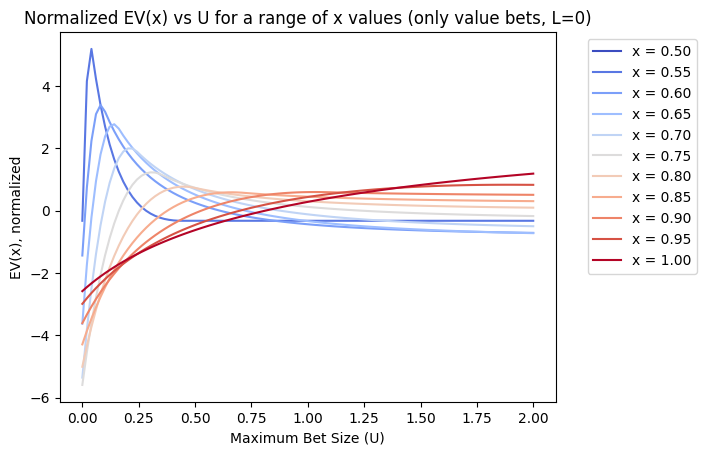
\includegraphics[width=\textwidth]{../parameter_analysis/images/ev_vs_U.png}
    \caption{Expected value of a value-betting hand $x$ versus the upper limit $U$ in Nash equilibrium. Each curve increases in $U$ up to some maximum, after which it decreases. This counterintuitive phenomenon is explained by strategic adjustments: as $U$ increases, the caller becomes more conservative (Appendix \ref{sec:parameter_analysis}).}
    \label{fig:ev_x_vs_U}
\end{figure}

The explanation lies in strategic interdependence: as $U$ increases, the bettor can make larger bets with their strongest hands, which forces the caller to become more conservative across \emph{all} bet sizes. This defensive adjustment by the caller harms the expected value of intermediate-strength hands, even though they're betting less. Only the very strongest hands (above a threshold greater than $v(U)$) benefit from the increased flexibility.

The complete analysis in Appendix \ref{sec:parameter_analysis} proves:
\begin{itemize}
    \item The bluffing threshold $x_2$ increases with $U$ (more hands bluff)
    \item For fixed hand $x \in [x_3, v(U)]$, the bet size $v^{-1}(x)$ decreases with $U$
    \item The calling cutoff $c(v^{-1}(x))$ increases with $U$ despite smaller bets
    \item There exists a threshold hand strength above which $EV(x)$ increases with $U$, and below which it decreases
\end{itemize}

These results demonstrate the rich strategic dynamics of LCP, where expanding betting options creates complex ripple effects throughout the equilibrium strategy profile.

\end{document}
